\chapter{Entorno experimental}

Con el objetivo de realizar la reconstrucción de cuerpos u objetos en modelos \gls{3d} se ha creado un pequeño entorno experimental donde realizar las pruebas.
El entorno está compuesto por el sensor Intel RealSense D435, montado en un trípode y con posición fija y un plato giratorio para las pruebas con objetos pequeños y rígidos.

En la Figura \ref{fig:entorno-experimental} podemos ver un objeto encima del plato giratorio y el sensor Intel Realsense D435 montado en el trípode.

\begin{figure}[h]
    \centering
    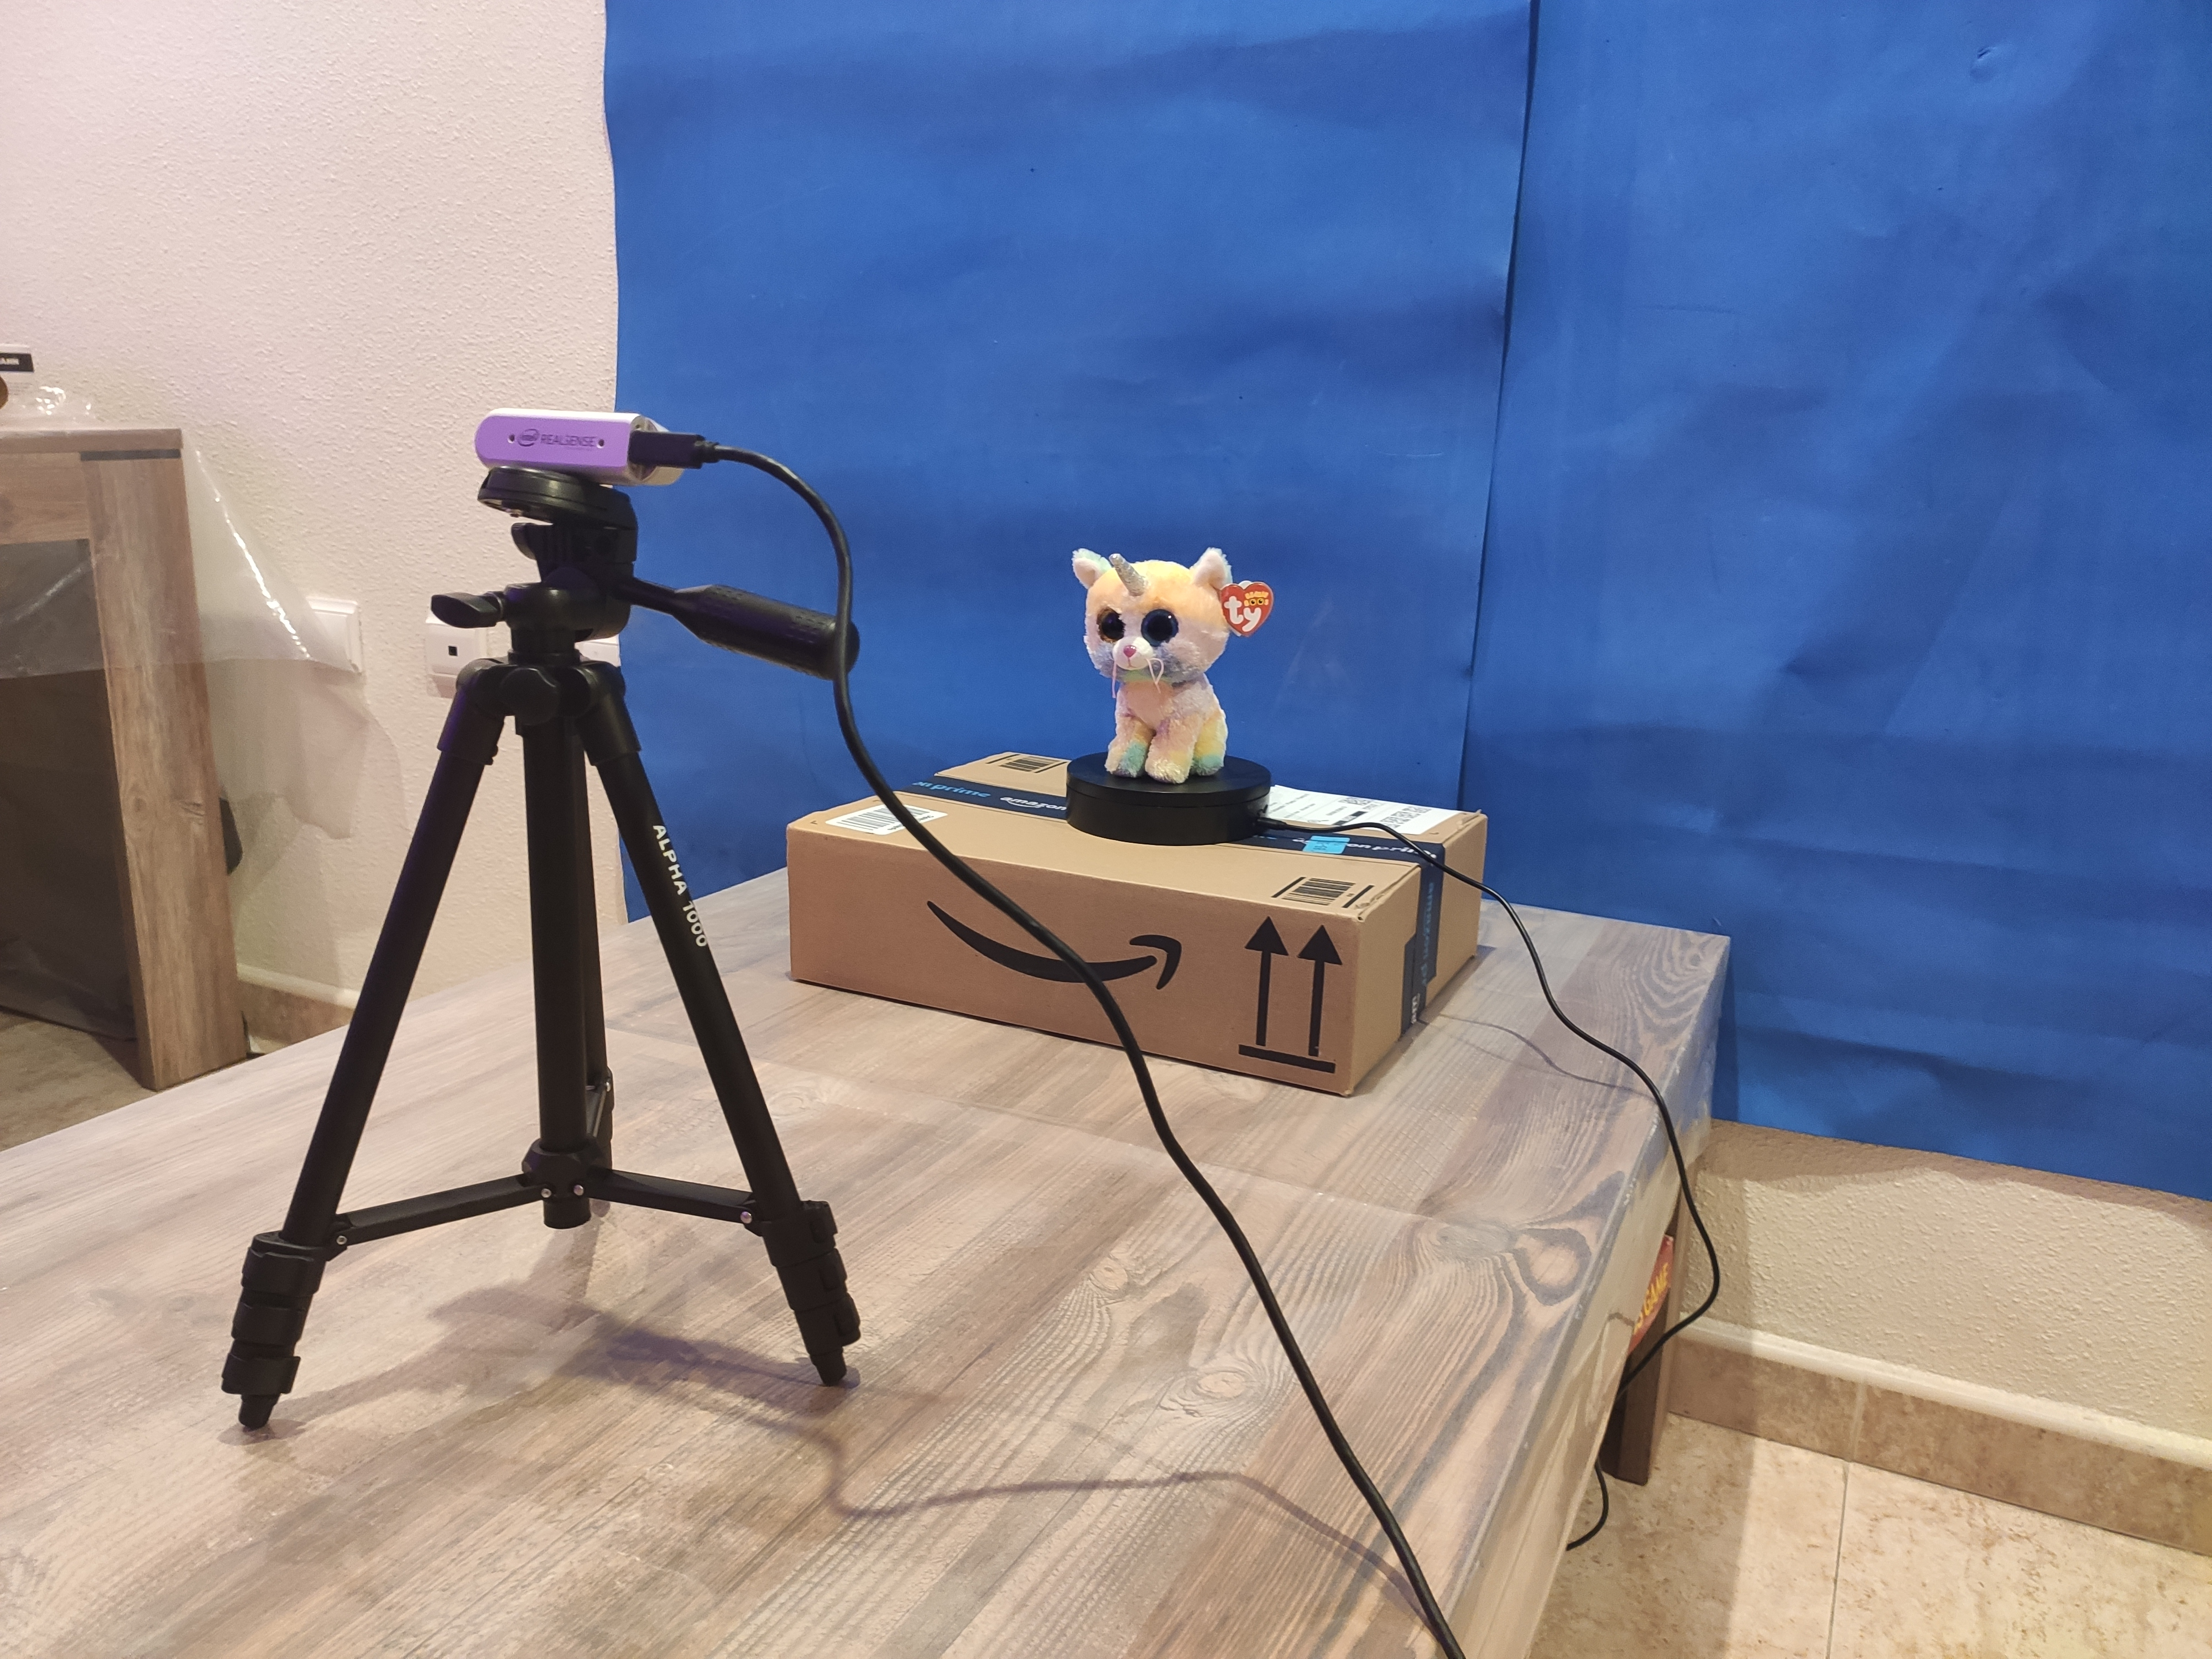
\includegraphics[width=\textwidth]{archivos/entorno-experimental-2.jpg}
    \caption{Entorno experimental.}
    \label{fig:entorno-experimental}
\end{figure}

El plato sobre el que está subido el objeto es un plato con velocidad fija que rota indefinidamente.
Utilizarlo facilita la tarea de reconstrucción \gls{3d} sobre los objetos ya que con el plato no necesitan ninguna interacción extra para rotar y ser capturados por todos los ángulos.
Esto ha facilitado la tarea de experimentación en objetos rígidos para su posterior prueba en cuerpos humanos.

La pared está cubierta con un panel de poliestireno azul con la finalidad de reducir ruido en la adquisición de datos, debido a que el sensor tiene pequeños fallos a la hora de identificar zonas concretas y muy detalladas y se llega a equivocar en el cálculo de profundidad de algunas zonas.
No obstante, aunque el poliestireno ha ayudado un poco, tampoco ha marcado gran diferencia, ya que esto ha seguido ocurriendo.

% \begin{figure}[h]
%     \centering
%     \begin{subfigure}[h]{0.5\textheight}
%     	\centering
%         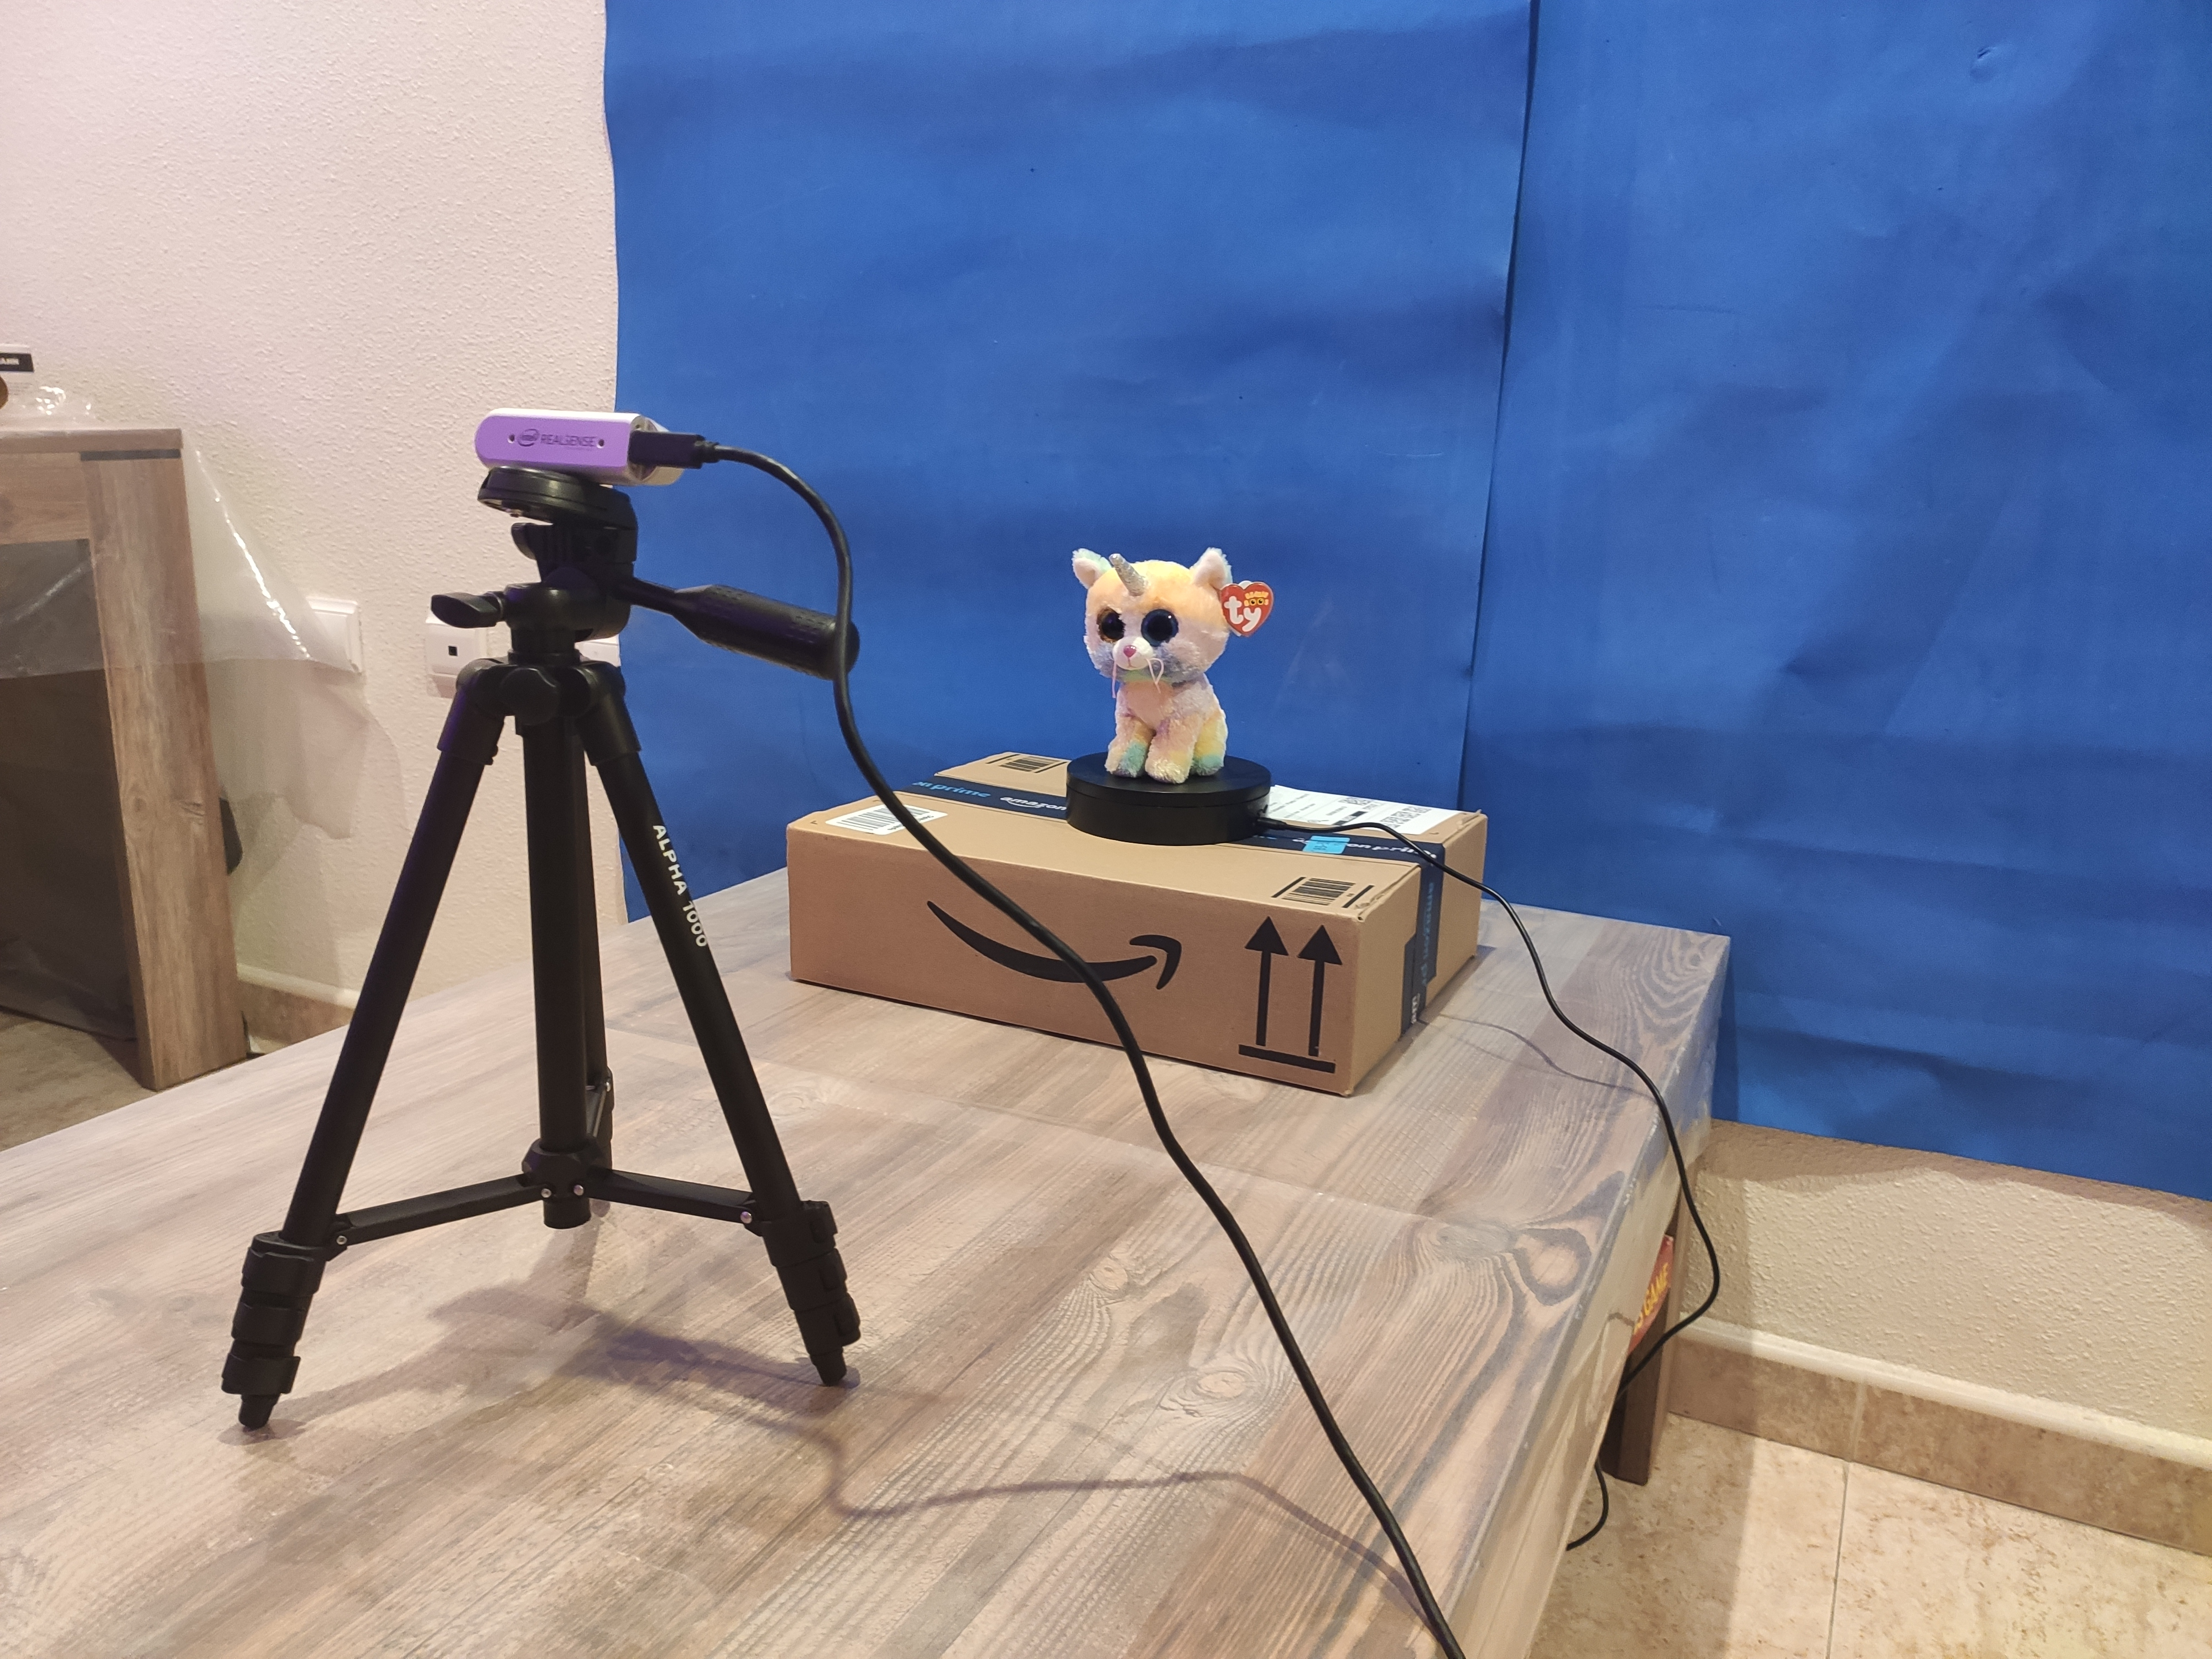
\includegraphics[width=\textwidth]{archivos/entorno-experimental-2.jpg}
%     \end{subfigure}
%     \begin{subfigure}[h]{0.6\textheight}
%     	\centering
%         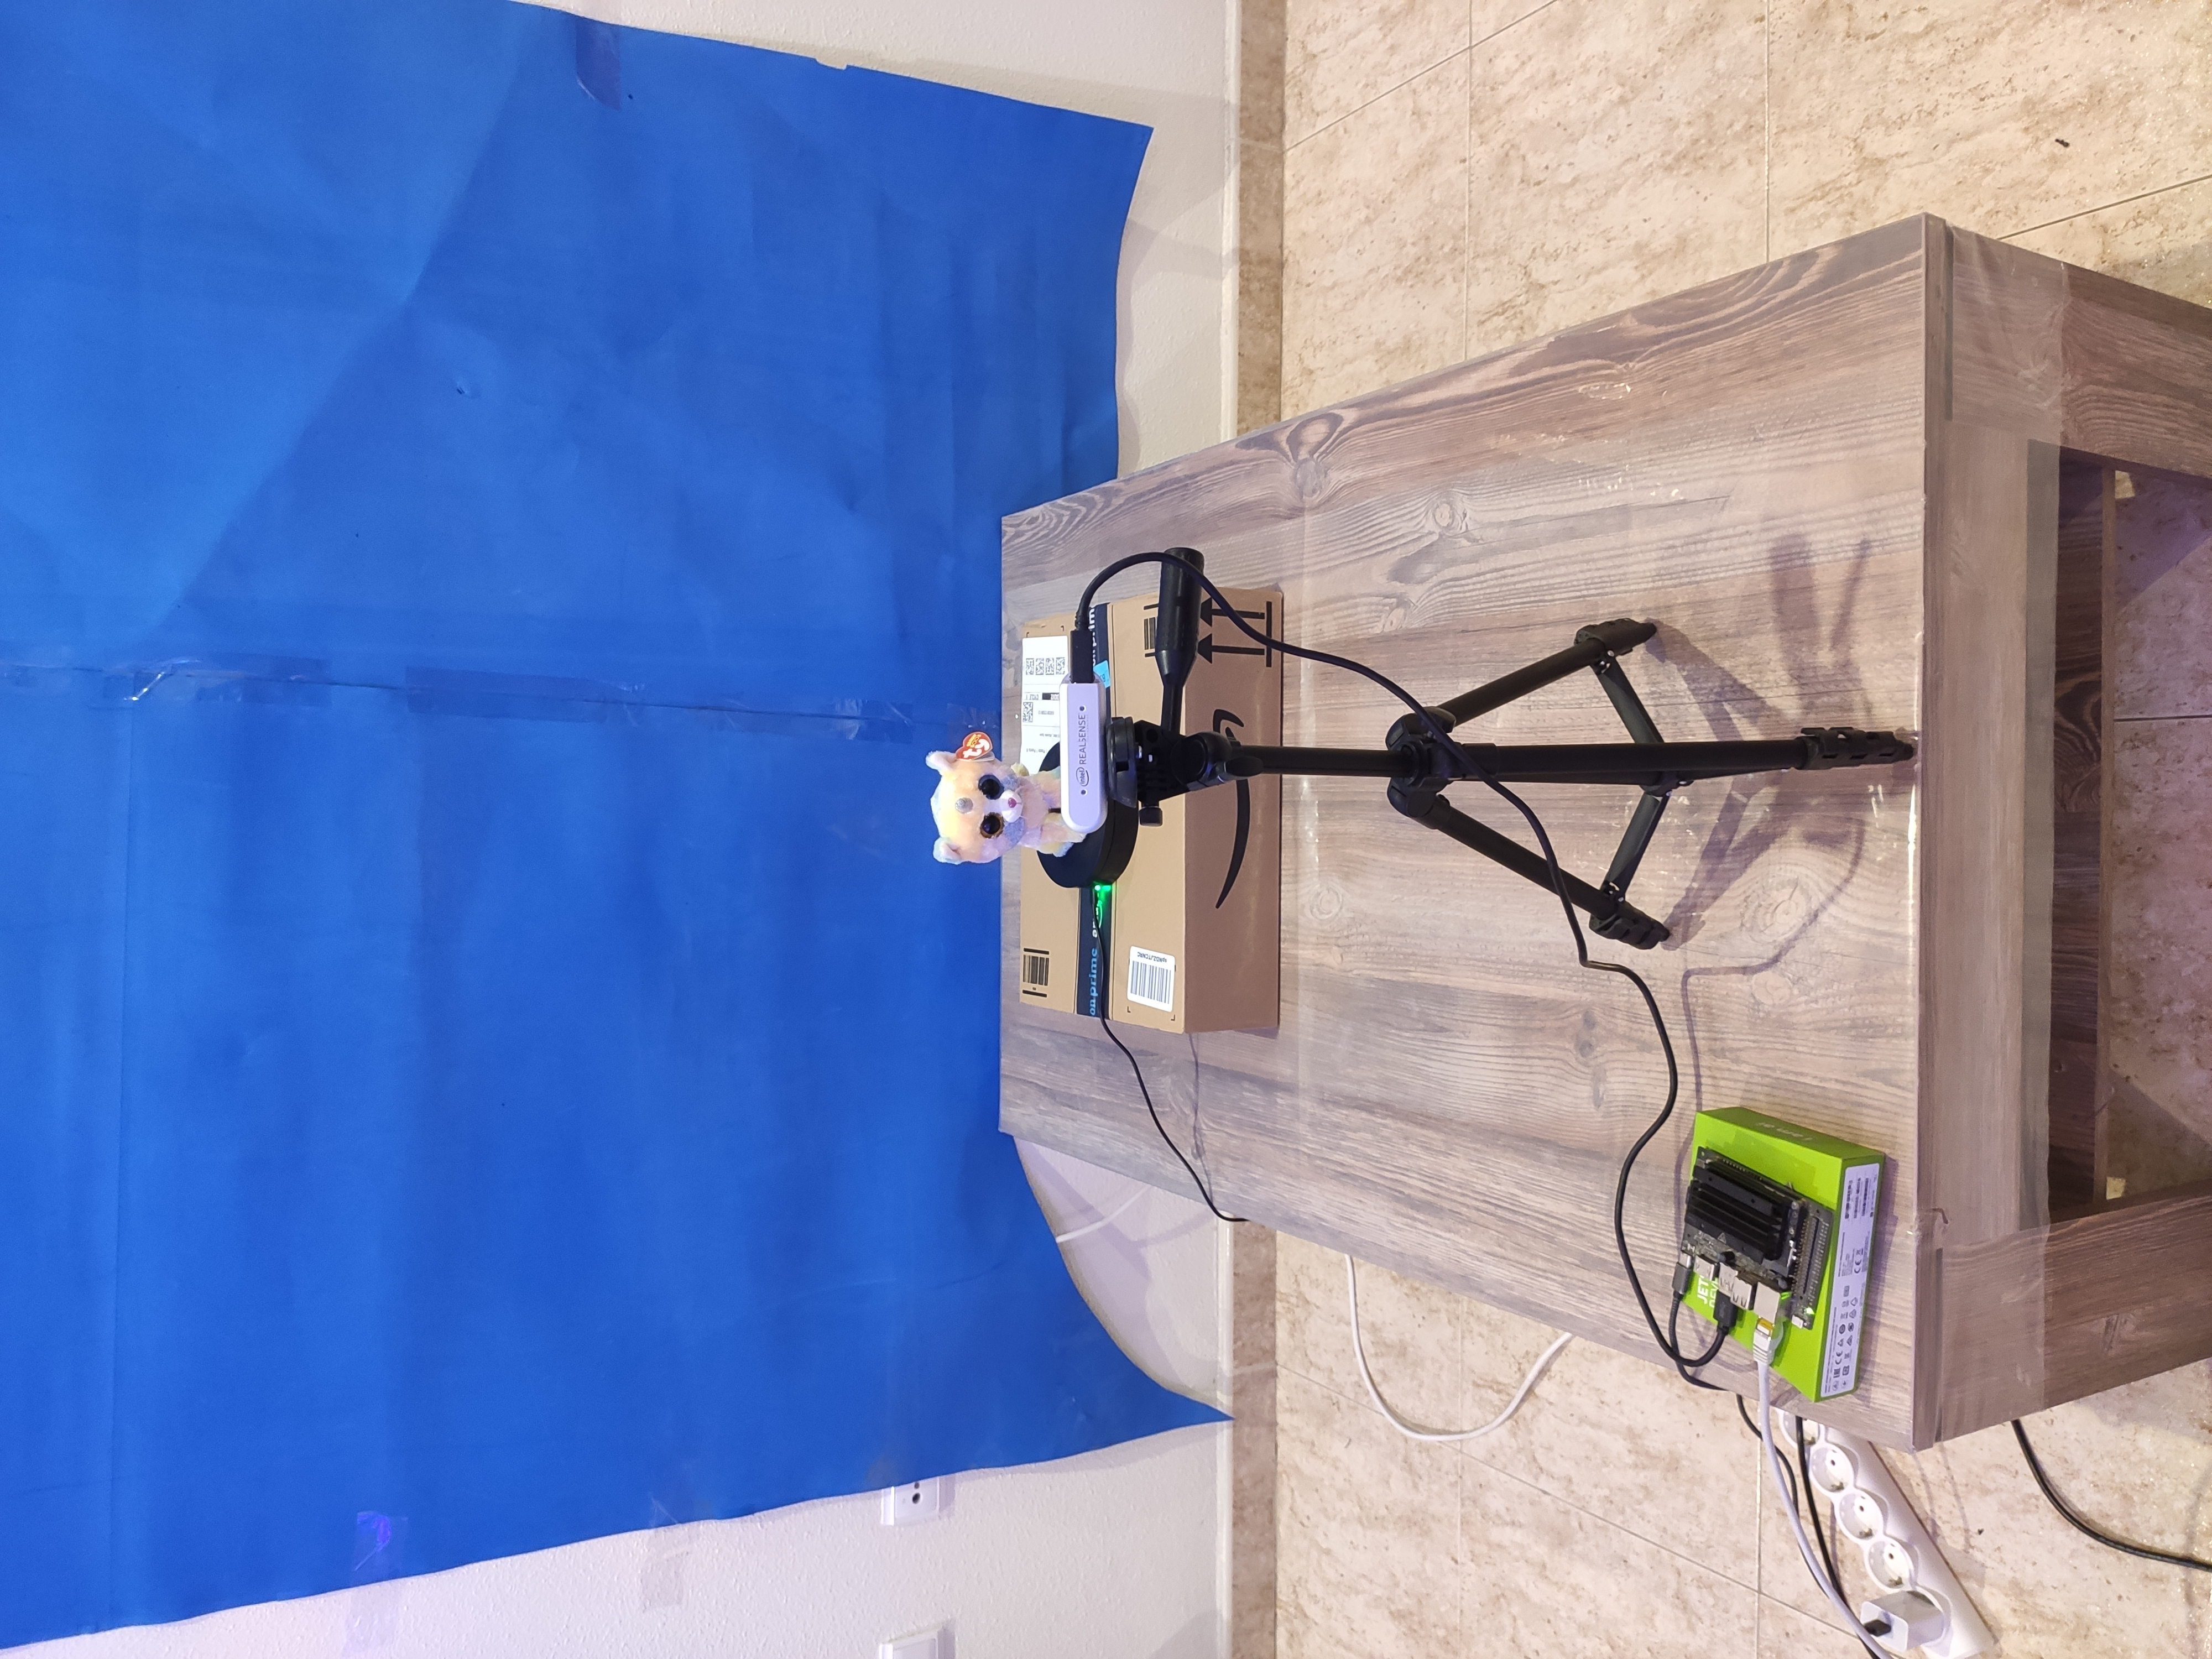
\includegraphics[width=\textwidth, angle=270]{archivos/entorno-experimental-1.jpg}
%     \end{subfigure}
%     \caption{Entorno experimental.}
%     \label{fig:entorno-experimental}
% \end{figure}